% allgem. Dokumentenformat
\documentclass[a4paper,12pt,headsepline]{scrartcl}
%Variablen welche innerhalb der gesamten Arbeit zur Verfügung stehen sollen
\newcommand{\titleDocument}{Bachelor Thesis}
\newcommand{\subjectDocument}{in Applied Computer Science}


\newcommand{\specialcell}[2][c]{%
	\begin{tabular}[#1]{c}
		#2
	\end{tabular}
}

\newcommand{\specialcellleft}[2][@{}l]{%
	\begin{tabular}[#1]{@{}l}
		#2
	\end{tabular}
}

\newcommand{\fixme}[1]{
	~\\
	\noindent
	\textbf{\textcolor{red}{FIXME: #1}}
	\\
}




% weitere Pakete
% Grafiken aus PNG Dateien einbinden
\usepackage{graphicx}

%for psuedo code
\usepackage[linesnumbered, ruled]{algorithm2e} 
%
\newcommand{\nosemic}{\SetEndCharOfAlgoLine{\relax}}% Drop semi-colon ;
\newcommand{\dosemic}{\SetEndCharOfAlgoLine{\string;}}% Reinstate
\newcommand{\pushline}{\Indp}% Indent
\newcommand{\popline}{\Indm\dosemic}% Undent
%\stackMath
%\[\def\stacktype{L}\setstackgap{L}{.4ex}
%x\mathrel{\stackon{\cup}{\scriptscriptstyle+}}y
%\mathrel{\stackon{\cup}{\scriptscriptstyle-}}z
%\]
%

% Eurozeichen einbinden
\usepackage[right]{eurosym}

\usepackage{ctable}

% Umlaute unter UTF8 nutzen
\usepackage[utf8]{inputenc}

% Zeichenencoding
\usepackage[T1]{fontenc}

\usepackage{lmodern}
\usepackage{fix-cm}

\usepackage{svg}

% floatende Bilder ermöglichen
%\usepackage{floatflt}

% mehrseitige Tabellen ermöglichen
\usepackage{longtable}

\usepackage{afterpage}

% Unterstützung für Schriftarten
%\newcommand{\changefont}[3]{ 
%\fontfamily{#1} \fontseries{#2} \fontshape{#3} \selectfont}

\setcounter{secnumdepth}{4}
\setcounter{tocdepth}{4}

% Packet für Seitenrandabständex und Einstellung für Seitenränder
\usepackage{geometry}
\geometry{left=3.5cm, right=2cm, top=2.5cm, bottom=2cm}

% Paket für Boxen im Text
\usepackage{fancybox}

% bricht lange URLs "schoen" um
\usepackage[hyphens,obeyspaces,spaces]{url}

% Paket für Textfarben
\usepackage{color}

% Mathematische Symbole importieren
\usepackage{amssymb}

% Writing text over arrows
\usepackage{mathtools}

% auf jeder Seite eine Überschrift (alt, zentriert)
%\pagestyle{headings}

% erzeugt Inhaltsverzeichnis mit Querverweisen zu den Kapiteln (PDF Version)
\usepackage[bookmarksnumbered,pdftitle={\titleDocument},hyperfootnotes=false]{hyperref} 
%\hypersetup{colorlinks, citecolor=red, linkcolor=blue, urlcolor=black}
%\hypersetup{colorlinks, citecolor=black, linkcolor= black, urlcolor=black}

% neue Kopfzeilen mit fancypaket
\usepackage{fancyhdr} %Paket laden
\pagestyle{fancy} %eigener Seitenstil
\fancyhf{} %alle Kopf- und Fußzeilenfelder bereinigen
\fancyhead[L]{\nouppercase{\leftmark}} %Kopfzeile links
\fancyhead[C]{} %zentrierte Kopfzeile
\fancyhead[R]{\thepage} %Kopfzeile rechts
\renewcommand{\headrulewidth}{0.4pt} %obere Trennlinie
%\fancyfoot[C]{\thepage} %Seitennummer
%\renewcommand{\footrulewidth}{0.4pt} %untere Trennlinie

% für Tabellen
\usepackage{array}

% Runde Klammern für Zitate
%\usepackage[numbers,round]{natbib}

% Festlegung Art der Zitierung - Havardmethode: Abkuerzung Autor + Jahr
\bibliographystyle{alphadin}

% Schaltet den zusätzlichen Zwischenraum ab, den LaTeX normalerweise nach einem Satzzeichen einfügt.
\frenchspacing

% Paket für Zeilenabstand
\usepackage{setspace}

% für Bildbezeichner
\usepackage{capt-of}

% für Stichwortverzeichnis
\usepackage{makeidx}

% für Listings
\usepackage{listings}
\lstset{numbers=left, numberstyle=\tiny, numbersep=5pt, keywordstyle=\color{black}\bfseries, stringstyle=\ttfamily,showstringspaces=false,basicstyle=\footnotesize,captionpos=b}
\lstset{language=java}

% Indexerstellung
\makeindex

% Abkürzungsverzeichnis
\usepackage[english]{nomencl}
\let\abbrev\nomenclature

% Abkürzungsverzeichnis LiveTex Version
\renewcommand{\nomname}{Abbreviations}
\setlength{\nomlabelwidth}{.25\hsize}
\renewcommand{\nomlabel}[1]{#1 \dotfill}
\setlength{\nomitemsep}{-\parsep}
\makenomenclature
%\makeglossary

% Abkürzungsverzeichnis TeTEX Version
% \usepackage[german]{nomencl}
% \makenomenclature
% %\makeglossary
% \renewcommand{\nomname}{Abkürzungsverzeichnis}
% \setlength{\nomlabelwidth}{.25\hsize}
% \renewcommand{\nomlabel}[1]{#1 \dotfill}
% \setlength{\nomitemsep}{-\parsep}

% Disable single lines at the start of a paragraph (Schusterjungen)
\clubpenalty = 10000
% Disable single lines at the end of a paragraph (Hurenkinder)
\widowpenalty = 10000
\displaywidowpenalty = 10000

\begin{document}
% hier werden die Trennvorschläge inkludiert
%hier müssen alle Wörter rein, welche Latex von sich auch nicht korrekt trennt bzw. bei denen man die genaue Trennung vorgeben möchte
\hyphenation{
Film-pro-du-zen-ten
Lux-em-burg
Soft-ware-bau-steins
zeit-in-ten-siv
}

%Schriftart Helvetica
%\changefont{phv}{m}{n}

% Leere Seite am Anfang
\newpage
\thispagestyle{empty} % erzeugt Seite ohne Kopf- / Fusszeile

% Titelseite %
% das Papierformat zuerst
%\documentclass[a4paper, 11pt]{article}

% deutsche Silbentrennung
%\usepackage[ngerman]{babel}

% wegen deutschen Umlauten
%\usepackage[ansinew]{inputenc}

% hier beginnt das Dokument
%\begin{document}


\thispagestyle{empty}

%\begin{figure}[t]
% \includegraphics[width=0.6\textwidth]{abb/fh_koeln_logo}
%\end{figure}

\begin{figure}[t]
 \centering
 
\includegraphics[width=0.6\textwidth]{abb/logo1}
~~~~~~~~~~
 
\includegraphics[width=0.20\textwidth]{abb/logo2}
\end{figure}


\begin{verbatim}


\end{verbatim}

\begin{center}
\Large{University of Bayreuth}\\
\end{center}


\begin{center}
\Large{Institute for Computer Science}
\end{center}
\begin{verbatim}








\end{verbatim}
\begin{center}
\doublespacing
\textbf{\LARGE{\titleDocument}}\\
\singlespacing
\begin{verbatim}

\end{verbatim}
\textbf{{~\subjectDocument}}
\end{center}
\begin{verbatim}

\end{verbatim}
\begin{center}

\end{center}
\begin{verbatim}






\end{verbatim}
\begin{flushleft}
\begin{tabular}{llll}
\textbf{Topic:} & & Integration of JPA-conform ORM-Implementations & \\
	& & in Hibernate Search & \\
& & \\
\textbf{Author:} & & Martin Braun <martinbraun123@aol.com>& \\
& & Matrikel-Nr. 1249080 & \\
& & \\
\textbf{Version date:} & & \today &\\
& & \\
\textbf{1. Supervisor:} & & Prof. Dr. Stefan Jablonski &\\
\textbf{2. Supervisor:} & & Prof. Dr. Bernhard Westfechtel &\\
\end{tabular}
\end{flushleft}

\pagebreak
~
\pagebreak

\begin{verbatim}






















\end{verbatim}

\begin{center}
	To my parents.
\end{center}

\afterpage{\null\newpage}
\pagebreak
~\\\\
\pagebreak
~


% römische Numerierung
%\pagenumbering{arabic}

% 1.5 facher Zeilenabstand
\onehalfspacing

% Einleitung / Abstract
% !TeX spellcheck = en_GB
\section*{Abstract}\label{abtract}
Every year, lecturer in the field of theoretical computer science or an related one face the task to create an exam exercise that tests if their students have understood the way of working of the Cocke-Younger-Kasami algorithm. Various implementations and small online tools of the CYK algorithm can be found, but none actually assists during the process of creating an exercise.\\
Therefore various algorithms to generate specifically suitable exercises have been designed and compared through their success rates. The different approaches for these algorithms involve the uniform randomly distribution of elements and the general Bottom-Up and Top-Down parsing approaches.\\
A GUI tool to automatically generate these exam exercises has been implemented. Its functionality contains that input parameters such as the count of variables, the count of terminals and the size of the word can be given. Suitable exam exercises are generated and one can be chosen for further modification and creation of the final exam exercise.\\


~~

\section*{Zusammenfassung}\label{zusammenfassung}
Jedes Jahr stehen Dozenten der theoretischen Informatik oder eines verwandten Bereiches vor der Aufgabe Klausuraufgaben zu erstellen, die prüfen ob ihre Studenten die Arbeitsweise des Cocke-Younger-Kasami-Algorithmus verstanden haben. Verschiedene Implementierungen und kleinere Online-Tools des CYK-Algorithmus gibt es bereits, aber Keines unterstützt beim Prozess des Erstellen einer Aufgabe.\\
Verschiedene Algorithmen wurden zuerst entworfen, um genau passende Aufgaben zu generieren und wurden anschließend auch miteinander über ihre Erfolgsrate verglichen. Die unterschiedlichen Ansätze für die Algorithmen beinhalten das gleichmäßig zufällige Verteilen von Elementen und die allgemeinen Ansätze des Bottom-Up und Top-Down Parsings.\\
Es wurde ein GUI-Tool implementiert um automatisch Klausuraufgaben zu generieren. Die Funktionalität des Tools beinhaltet, dass Eingabewerte wie die Anzahl der Variablen, die Anzahl der Terminale und die Wortlänge gemacht werden können. Geeignete Klausuraufgaben werden automatisch generiert von denen Eine für weitere Modifikation und letztendlich für die Klausuraufgabenerstellung ausgewählt wird.\\



\pagebreak



% einfacher Zeilenabstand
\singlespacing

% Inhaltsverzeichnis anzeigen
\newpage
\tableofcontents
\addcontentsline{toc}{section}{Abstract}
~
\pagebreak

% das Abbildungsverzeichnis
%\newpage
% Abbildungsverzeichnis soll im Inhaltsverzeichnis auftauchen
%\addcontentsline{toc}{section}{List of figures}
% Abbildungsverzeichnis endgueltig anzeigen
%\offigures

% das Tabellenverzeichnis
%\newpage
% Abbildungsverzeichnis soll im Inhaltsverzeichnis auftauchen
%\addcontentsline{toc}{section}{Tabellenverzeichnis}
% \fancyhead[L]{Abbildungsverzeichnis / Abkürzungsverzeichnis} %Kopfzeile links
% Abbildungsverzeichnis endgueltig anzeigen
%\listoftables

%% WORKAROUND für Listings
%\makeatletter% --> De-TeX-FAQ
%\renewcommand*{\lstlistoflistings}{%
%  \begingroup
%    \if@twocolumn
%      \@restonecoltrue\onecolumn
%    \else
%      \@restonecolfalse
%    \fi
%    \lol@heading
%    \setlength{\parskip}{\z@}%
%    \setlength{\parindent}{\z@}%
%    \setlength{\parfillskip}{\z@ \@plus 1fil}%
%    \@starttoc{lol}%
%    \if@restonecol\twocolumn\fi
%  \endgroup
%}
%\makeatother% --> \makeatletter
% das Listingverzeichnis
%\newpage
% Listingverzeichnis soll im Inhaltsverzeichnis auftauchen
%\addcontentsline{toc}{section}{Listingverzeichnis}
%\fancyhead[L]{Abbildungs- / Tabellen- / Listingverzeichnis} %Kopfzeile links
%\renewcommand{\lstlistlistingname}{Listingverzeichnis}
%\lstlistoflistings
%%%%

% das Abkürzungsverzeichnis
%\newpage
% Abkürzungsverzeichnis soll im Inhaltsverzeichnis auftauchen
%\addcontentsline{toc}{section}{Abkürzungsverzeichnis}
% das Abkürzungsverzeichnis entgültige Ausgeben
%\fancyhead[L]{Abkürzungsverzeichnis} %Kopfzeile links
%\nomenclature{UGC}{User Generated Content}
\nomenclature{CSS}{Cascading Style Sheets}
\nomenclature{JS}{JavaScript}
\nomenclature{SQL}{Structured Query Language}
\nomenclature{GPL}{GNU General Public License}
\nomenclature{GNU}{GNU is not Unix}
\nomenclature{LGPL}{GNU Lesser General Public License}
\nomenclature{XMPP}{Extensible Messaging and Presence Protocol}
\nomenclature{IM}{Instant Message}
\nomenclature{CMS}{Content Management System}
\nomenclature{RSS}{Really Simple Syndication}
\nomenclature{JSON}{JavaScript Object Notation}
\nomenclature{HTML}{Hypertext Markup Language}
\nomenclature{TDD}{Test-driven development}
\nomenclature{GUI}{Graphical User Interface}
\nomenclature{KPI}{Key Performance Indicator}
\nomenclature{WWW}{World Wide Web}
\nomenclature{OCR}{Optical Character Recognition}
\nomenclature{ERM}{Entity Relationship Modell}

%\printnomenclature

% Definiert Stegbreite bei zweispaltigem Layout
\setlength{\columnsep}{25pt}

%%%%%%% EINLEITUNG %%%%%%%%%%%%
%\twocolumn
\newpage
\fancyhead[L]{\nouppercase{\leftmark}} %Kopfzeile links

% 1,5 facher Zeilenabstand
\onehalfspacing

% einzelne Kapitel
% !TeX spellcheck = en_GB

\section{Introduction}\label{Introduction}

\noindent What has already been done in this area? Why are you doing this?\\ 

\noindent Let there be a grammar $G=(V,\ \Sigma,\ S,\ P)$ in Chomsky Normal Form (CNF).\\
$V$ is a finite set of variables. \\
$\Sigma$ is an alphabet. \\
$S$ is the starting symbol and $S \in V$. \\
$P$ is a finite set of rules: $P \subseteq V \times (V \cup \Sigma)^{*}$. $G$ is in CNF and therefore, more specifically, it holds:  $P\ \subseteq\ V \times (V^{2} \cup \Sigma)$.\\
 
\noindent For simplification the default definitions hold:
\begin{itemize}
	\item $V = \{A, B, ...\}$
	\item $(V^2 \cup\ \Sigma)^{*}=\{a, b, ...\} \cup \{AB, BS, AC, ... \}$
\end{itemize}

\noindent Let there be a word $w \in \Sigma^*$, a language $L(G)$ and a grammar $G$ in CNF. 

\subsection{Forward Problem vs. Backward Problem}

\noindent\textbf{Forward Problem ($G \xrightarrow[]{derivation} w$):}\\
Informal definition: "Forming a derivation from a root node to a final sentence."  [Duda 8.6.3 page 426]\\
Input: Grammar $G$ in CNF.\\
Output: Derivation $d$ that shows implicitly $w \subseteq L$.\\

\noindent\textbf{Backward Problem = Parsing ($w\overset{?}{\subseteq}L(G)$):}\\
Informal definition: "Given a particular $w$, find a derivation in $G$ that leads to $w$. This process, called parsing, is virtually always much more difficult than forming a derivation."  [Duda 8.6.3 page 426]\\
Input: $w$ and a grammar $G$ in CNF.\\
Output: $w \subseteq L(G) \Longrightarrow$ derivation $d$.\\

\subsection{Parsing: Bottom-Up vs Top-Down}

\noindent\textbf{Bottom-Up:} Bottom-Up parsing is "the general method used in the Cocke-Younger-Kasami(CYK) algorithm, which fills a parse table from the "bottom up"." (Bottom up means starting from the leaves.) [Duda 8.6.3 page 426]\\

\noindent\textbf{Top-Down:} "Top-Down parsing starts with the root node and successively applies productions from $P$, with the goal of finding a derivation of the test sentence $w$. Because it is rare indeed that the sentence is derived in the first production attempted, it is necessary to specify some criteria to guide the choice of which rewrite rule to apply. Such criteria could include beginning the parse at the first (left) character in the sentence (i.e., finding a small set of rewrite rules that yield the first character), then iteratively expanding the production to derive subsequent characters, or instead starting at the last (right) character in the sentence." [Duda 8.6.3 page 428]\\

\subsection{Scope of this thesis}

The starting point of this thesis was to get a command line interface (CLI) tool to automatically generate $exercises = (grammar,\ word,\ parse\ table,\ derivation\ tree)$, which are used to test if the students have understood the way of working of the CYK algorithm. A scoring model is used to evaluate the generated exercises regarding their usability in an exam.\\

\noindent This alone doesn't meet the requirements for being an adequate topic for a bachelor thesis.
Therefore the task of finding a clever algorithm to get exercises with a high chance of being usable as an exam exercise was added.\\

\pagebreak

%% !TeX spellcheck = en_GB

\section{Technology Overview}\label{TechnologyOverview}

\pagebreak

% !TeX spellcheck = en_GB

\section{Simple Scoring Model}

\noindent Short preface to the rationale about the scoring model. 

\subsection{Elimination Criteria and Selection Criteria}

\noindent Success rates: 
Producibility: $w \subseteq L(G)$\\
Grammar restricitons: $n=|w|$, maxNumberOfVarsPerCell; \textbf{Delete SuccessRatesGrammarRestrictions class. Move maxNumberOfVarsPerCell to exam restrictions class and use $n$ only as parameter.} \\
Exam restrictions: rightCellCombinationsForcedCount, maxSumOfProductions, maxSumOfVarsInPyramid\\

\noindent Picture of used scoring model without weights here. Maybe one picture together with the next subsection. 

\subsection{Weighting of the criteria}

\noindent Picture of the final used scoring model with weights here. 

\subsection{Direct Ranking vs. Preference Analysis vs. ...}

What method is used to compare the results out of the scoring model.\\
Direct Ranking is the simplest way.

\pagebreak

% !TeX spellcheck = en_GB

\section{Algorithms}\label{algorithms}
\noindent Analogue to the script: \\
grammar $G=(V,\Sigma , S, P)$.\\
$V$ is a finite set of variables. \\
$\Sigma$ is an alphabet. \\
$S$ is the starting symbol and $S\ \epsilon\ V$. \\
$P$ is a finite set of rules: $P\ \subseteq\ V \times\ (V \cup\ \Sigma)^{*}$. \\ 
LHSE and RHSE are sets that shouldn't be defined. It is possible to have context free grammars(cfgs) with other kind of combinations.\\
$LHSE$ is finite set of left hand side elements: $LHSE = V$.\\
$RHSE$ is finite set of right hand side elements: $RHSE = (V \cup\ \Sigma)^{*}$.\\
$G.P.RHSE$ allows access to $RHSE$.\\
Variables that are of type set begin with a upper case letter.\\
$p.rhse$ allows access to the one specific $rhse$ of the specific production $p$.\\
So $P$ is a finite set of rules: $P\ \subseteq\ LHSE \times\ RHSE$. \\
Multisets allow duplicate elements. Notation of a multiset is done via the index b: $multiset_b$\\
pyramid is a structure where one $cell_{i,j}$ holds a set  $Cell_{i,j} = \{v\ |\ v\ \epsilon\ V\}$. If initialised each $cell_{i,j}$ holds $Cell_{i,j} = \emptyset $, which is named $empty\ pyramid$. $cell_{i+1,j} = cellDown;$ $cell_{i,j} = cellUpperLeft;\ cell_{i+1,j+1} = cellUpperRight;  $ \\
RHSEs are terminals like "a, b, ..." and compound variables like "AB, AC, ...". \\
LHSEs are variables like "A, B, ...".\\


\begin{figure}[h]
	\centering
	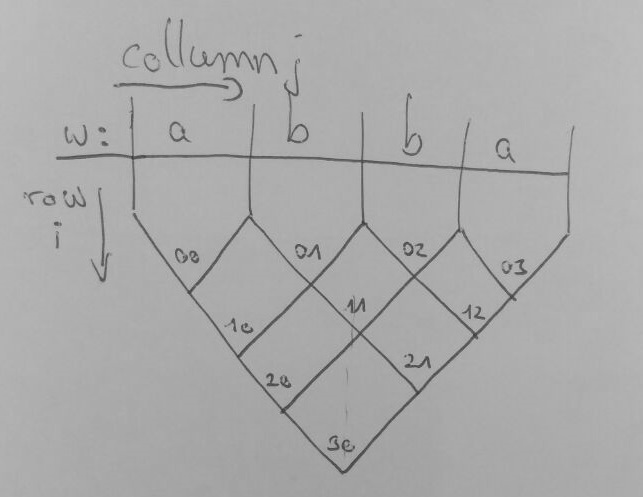
\includegraphics[width=0.7\textwidth]{abb/DataStructurePyramid}
\end{figure}

 \pagebreak 
 
\frame{
	\begin{algorithm}[H] %or another one check
		\caption{distributeRhseRandomly}
		\label{distributeRhseRandomly}
		\SetAlgoLined
		\KwIn{ $G,\ Rhse \subseteq\ RHSE,\ 0\leq minCount\leq maxCount\leq \mid G.V\mid$}
		\KwOut{$Grammar\ G\ with\ randomly\ distributed\ Rhse's.$}
		\ForEach {$rhse\ in\ Rhse$}{
			$addCount$ = $random(minCount, maxCount)$\;
			$VarsToAddTo = randomSubSet(addCount,\ LHSE)$\;
			
		
			\ForEach{var in VarsToAddTo}{
				$G.P = G.P\ \cup\ \{ "var\longrightarrow rhse" \} $\;	
			}
		}
		\Return $G$;
	\end{algorithm}
}
.\\
.\\
\frame{
	\begin{algorithm}[H] %or another one check
		\caption{GeneratorGrammarDiceRollMartens}
		\label{GeneratorGrammarDiceRollMartens}
		\SetAlgoLined
		\KwIn{ $word \in \Sigma^{*},\ V,\ \Sigma,\ S,\ P = \emptyset,\ minCount\Sigma,\ maxCount\Sigma,\ $ $ minCountVarComp,\ maxCountVarComp $ }
		\KwOut{$G$}
		
		$G=(V,\Sigma , S, P)$\;
		$G = distributeRhseRandomly(G,\ \Sigma,\ minCount\Sigma,\ maxCount\Sigma ) $\;
		$pyramid = CYK.calculatePyramid(G,\ word)$\;
		\ForEach{$cell_{i+1,j}\ in\ pyramid\ \wedge\ i>0$}{
			$VarComp = \{XY\ |\ X \in cellUpperLeft\ \wedge\ Y \in cellUpperRight \}$\;
			\ForEach{$vc\ in\ VarComp$}{
				\While{$cell_{wordLength+1,0} = \emptyset$}{
					$distributeRhseRandomly(G,\ vc,\ minCountVarComp,\ $ $maxCountVarComp ) $\;
					$pyramid = CYK.calculatePyramid(G,\ word)$\;	
				}
			}
		}
		\Return $G$\;
		\footnotetext{Line 3: Fills the i=0 row of the pyramid.\\
			\noindent Line 4: = foreach cellDown, but skipping the first row of the pyramid.
		}
	\end{algorithm}
}

 \pagebreak 
 
 
\frame{
 	\begin{algorithm}[H] %or another one check
 		\caption{checkRightCellCombination}
 		\label{checkRightCellCombination}
 		\SetAlgoLined
 		\KwIn{$ cellDown\subseteq V \,\ cellUpperLeft\subseteq V,\ cellUpperRight\subseteq V,\ G.P $ }
 		\KwOut{$varsThatForce\subseteq V$}
 		$isForced = false$\;
 		$VarsThatForce = \emptyset$\;
 		$VarComp = \{XY\ |\ X \in cellUpperLeft\ \wedge\ Y \in cellUpperRight \}$\;
 		\ForEach{$v\ in\ cellDown$}{
 			$VProd = \{p\ |\ p \in G.P\ \wedge\ p.lhse = v \}$\;
 			$VRhse = \{vRhse\ |\ vRhse \in VProd.RHSE \} $\;
 			\If{$VarComp \nsubseteq VRhse$}{
 				$isForced = true$\;
 				$VarsThatForce = VarsThatForce\ \cup\ v$\;
 			}			
 		}
 		\Return $VarsThatForce$\;
 	\end{algorithm}
}
\pagebreak


\frame{
 	\begin{algorithm}[H] %or another one check
 		\caption{checkRightCellCombinationForced}
 		\label{checkRightCellCombinationForced}
 		\SetAlgoLined
 		\KwIn{$ pyramid,\ G,\ minCountForced $ }
 		\KwOut{$G$}
 		$countForced = 0$\;
 		$isForced = true$\;
 		$varsThatForce = empty\ pyramid$\;
 		\ForEach{$cell_{i+1,j}\ in\ pyramid\ \wedge\ i>1 $}{
 			$varComp = \{XY\ |\ X\ \epsilon\ Cell_{i,j}\ \wedge\ Y\ \epsilon\ Cell_{i+1,j+1} \}$\;
 			
 			
 			
 			$ $\;
 		}
 		\Return $isForced,\ countForced,\ varsThatForce$\;
 		\footnotetext{Line 3: $i>1 \rightarrow$ the upper two rows aren't included, because they would produce trivial cases that fulfil the restriction always. 
 		}
 	\end{algorithm}
}
 
\pagebreak
 
\lstset{language=java}
\begin{lstlisting}[frame=htrbl, caption={distributeDiceRollRightHandSideElements}, 
label={lst:distributeDiceRollRightHandSideElements}]
Algorithm: distributeDiceRollRightHandSideElements
Input: grammar, setRhse, minCount, maxCount, listVars;
Output: grammar;

for(RightHandSideElement rhse : setRhse){
	// countWillBeAdded is between [minCount, maxCount]. 
	countWillBeAdded = diceRoll();
	while(listVars.size() > countWillBeAdded){
		Remove one variable of listVars via dice roll;
	}
	for(Variable varLeft : listVars){
		// An exception is thrown if the production 
		// already exists.
		grammar.addProduction "varLeft --> rhse";
	}
}
return grammar;
\end{lstlisting}


\lstset{}
\begin{lstlisting}[frame=htrbl, caption={distributeDiceRollRightHandSideElementsShort}, 
label={lst:distributeDiceRollRightHandSideElementsShort}]
Algorithm: distributeDiceRollRightHandSideElements
Input: grammar G, setRhse, minCount, maxCount, setGrammarVars;
Output: grammar;

foreach rhse in setRhse { 
	countWillBeAdded = dice roll a number within [minCount, maxCount];
	setVarsToAddRhse = {}dice roll countWillbeAdded to times vars from 	
		setGrammarVars that get the rhse added to;
	foreach var in setVarsToAddRhse {
		add production "var --> rhse" to grammar;
	}
}
return grammar;
\end{lstlisting}

\lstset{language=java}
\begin{lstlisting}[frame=htrbl, caption={CYK.calculateSetVAdvanced}, 
label={lst:CYK.calculateSetVAdvanced}]
Algorithm: CYK.calculateSetVAdvanced
Input: grammar, word;
Output: Set<VariableK>[][] cYKMatrix;

Set<VariableK>[][] cYKMatrix = new Set<VariableK>[wordSize][wordSize];
cYKMatrix = calculateCYKMatrix;
return cYKMatrix;
\end{lstlisting}

\pagebreak

\lstset{language=java}
\begin{lstlisting}[frame=htrbl,caption={GeneratorGrammarDiceRollTopDownMartens}, 
label={lst:GeneratorGrammarDiceRollTopDownMartens}]
Algorithm: GeneratorGrammarDiceRollTopDownMartens
Input: word, settings;
Output: grammar;
Note: Keep in mind that the setV matrix is a upper right matrix. But the
description of how the algorithm works is done, as if the setV pyramid 
points downwards (reflection on the diagonal + rotation to the left).
Regarding one cell, its upper left cell and its upper right cell 
are looked at. setV[i][j] = down cell. setV[i + 1][j] = upper right cell
setV[i][j - 1] = upper left cell. With wordSize = 5, the visited indexes 
are as following: [01->12->23->34; 02->13->24; 03->14; 04;]

Grammar grammar = new Grammar();
// Part1: Distribute the terminals.
grammar = distributeDiceRollRightHandSideElements(
	grammar, settingsTerminals, minCountTerminals, 
	maxCountTerminals, settingsListVariables);
// Part2: Distribute the compound variables.
Set<VariableKWrapper>[][] setVAdvanced;
// Fill the diagonal of the matrix with:
setVAdvanced = CYK.calculateSetVAdvanced( grammar, word );
for(Cell cellToBeVisited : setVAdvanced){
	setVariableCompound = calculate all the possible tupels of 
		({varLeft}, {varRight});
	for(VariableCompound varComp : setVariableCompound){
		// Because of dice rolling anyways and lots of grammars 
		// being generated, no varComp is added if the production
		// already exists.
		grammar = distributeDiceRollRightHandSideElements(
			grammar, varComp, minCountVarComp, 
			maxCountVarComp, settingsListVariables);
		setVAdvanced = CYK.calculateSetVAdvanced( grammar, word );
	}
}
return grammar;
// Forgot the while cell not empty do this from line 21 to line 33;
\end{lstlisting}

\pagebreak

\lstset{language=java}
\begin{lstlisting}[frame=htrbl,caption={GeneratorGrammarDiceRollOnly}, 
label={lst:GeneratorGrammarDiceRollOnly}]
Algorithm: GeneratorGrammarDiceRollOnly
Input: settings;
Output: grammar;
Note: A lot of productions are generated, that later on are not needed
for parsing the specific word.

Grammar grammar = new Grammar();
// Part1: Distribute the terminals.
grammar = distributeDiceRollRightHandSideElements(
	grammar, settingsTerminals, minCountTerminals, 
	maxCountTerminals, settingsListVariables);
// Part2: Distribute the compound variables.
Set<Variables> vars = settings.getVariables();
Set<VariablesCompound> setVarComp;
setVarComp = calculate all the possible tupels of ({vars}, {vars});
grammar = distributeDiceRollRightHandSideElements(
	grammar, settingsTerminals, minCountVariableCompound, 
	maxCountVariableCompound, setVarComp);
return grammar
\end{lstlisting}

\pagebreak

\lstset{language=java}
\begin{lstlisting}[frame=htrbl,caption={GeneratorGrammarDiceRollOnlyBias}, 
label={lst:GeneratorGrammarDiceRollOnlyBias}]
Algorithm: GeneratorGrammarDiceRollOnlyBias
Input: settings;
Output: grammar;
Note: A lot of productions are generated, that later on are not needed
for parsing the specific word.

Grammar grammar = new Grammar();
// Distribute the terminals.
grammar = distributeDiceRollRightHandSideElementsBias(
	grammar, settingsTerminals, settingsMinCountTerminals, 
	settingsMCountTerminals, settingsListVars, settingsFavouritism);

// Distribute the compound variables.
Set<VariablesCompound> setVarComp;
setVarComp = calculate all the possible tupels of ({vars}, {vars});
grammar = distributeDiceRollRightHandSideElementsBias(
	grammar, varComp, settingsMinCountVars,
	settingsMaxCountVars, settingsListVars, settingsFavouritism);
return grammar;
\end{lstlisting}

\pagebreak

\lstset{language=java}
\begin{lstlisting}[frame=htrbl,caption={distributeDiceRollRightHandSideElementsBias}, 
label={lst:distributeDiceRollRightHandSideElementsBias}]
Algorithm: distributeDiceRollRightHandSideElementsBias
Input: grammar, setRhse, minCount, maxCount, listVars, favouritismList;
Output: grammar;
Note: Because of dice rolling anyways and lots of grammars being 
generated, no rhse is added if the production already exists.

// Calculate the bloated varSet.
List<Variable> varsBloated;
for(Variables varTemp :  settings.getVariables()){
	tempFavour = randomly pick favouritism[i];
	varsBloated.add({tempFavour times varTemp});
	favouritism.remove(tempFavour);
}
// Because of dice rolling anyways and lot of grammars being generated, 
// just no rhse is added if the production already exists.
grammar = distributeDiceRollRightHandSideElements( grammar,
	varsBloated, minCount, maxCount, listVars );
return grammar;
\end{lstlisting}

\frame{
	\begin{algorithm}[H] %or another one check
		\caption{distributeDiceRollRightHandSideElementsBias}
		\label{distributeDiceRollRightHandSideElementsBias}
		\SetAlgoLined
		\KwIn{ $G,\ rhse \subseteq\ RHSE,\ 0\leq minCount\leq maxCount\leq\ \mid G.V\mid,\ favouritism = \{x\ |\ x\ \epsilon\ \mathrm{N}\ \wedge\ |favouritism| = |G.V| \}$}
		\KwOut{$G$}
		
		$favour = \{(v,\ f )\ |\ v\ \epsilon\ V \wedge\ f\ \epsilon\ favouritism\  \wedge\ tupel\ are\ created\ via\ dice\ roll \}$\;
		$varsBloated_b = \emptyset $\;
		\ForEach{fav in favour}{
			$varsBloated_b = varsBloated_b\ \biguplus\ \{ v^{f} \}$\;
		}
		\Return $distributeDiceRollRhse(
		G ,\ MISTAKEHEREvarsBloated_b,\ minCount,\ maxCount\ )$\;
		
		Still working on. One more Pprameter needed for distributeDiceRollRighthandSideElement. Parameter V that defines the variables the rhse are added to. OR make this algorithm independent.
		\footnotetext{Line 6: Note that $varsBloated_b$ is a multiset, but should actually be a set. Exceptions causing a duplicate production to
		the grammar are not relevant because G.P is a set. }
	\end{algorithm}
}

\pagebreak
\noindent Description of the checks here. \\
\noindent All test of the GrammarValidityChecker class are based on the simple setV matrix. \\

\noindent  isValid = isWordProducible \&\& isExamConstraints \&\& isGrammarRestrictions\\

\noindent  isWordProducible = CYK.algorithmAdvanced()\\

\noindent  isExamConstraints = isRightCellCombinationsForced \&\& isMaxSumOfProductionsCount \&\& isMaxSumOfVarsInPyramidCount \&\& countRightCellCombinationsForced \\

\noindent isGrammarRestrictions = isSizeOfWordCount \&\& isMaxNumberOfVarsPerCellCount \\

\lstset{language=java}
\begin{lstlisting}[frame=htrbl, caption={checksumOfProductions}, 
label={lst:checksumOfProductions}]
Algorithm: checksumOfProductions
Input: grammar, maxSumOfProduction;
Output: isSumOfProductions;

return grammar.getProductionsAsList().size() <= maxSumOfProductions; 
\end{lstlisting}

\pagebreak
\lstset{language=java}
\begin{lstlisting}[frame=htrbl, caption={checkMaxNumberOfVarsPerCell}, 
label={lst:checkMaxNumberOfVarsPerCell}]
Algorithm: checkMaxNumberOfVarsPerCell
Input: setVSimple, maxNumberOfVarsPerCell;
Output: isMaxNumberOfVarsPerCell;
Note: Checking for maxNumberOfVarsPerCell <= zero isn't allowed;

int tempMaxNumberOfVarsPerCell = 0;
int wordLength = tempSetV[0].length;
for ( int i = 0; i < wordLength; i++ ) {
	for ( int j = 0; j < wordLength; j++ ) {
		if ( tempSetV[i][j].size() > numberOfVarsPerCell ) {
			numberOfVarsPerCell = tempSetV[i][j].size();
		}
	}
}
return tempMaxNumberOfVarsPerCell <= maxNumberOfVarsPerCell;
\end{lstlisting}

\pagebreak

\lstset{language=java}
\begin{lstlisting}[frame=htrbl, caption={checkMaxSumOfVarsInPyramid}, 
label={lst:checkMaxSumOfVarsInPyramid}]
Algorithm: checkMaxSumOfVarsInPyramid
Input: setVSimple, maxSumOfVarsInPyramid;
Output: isMaxSumOfVarsInPyramid;

// put all vars of the matrix into one list and use its length.
List<Varaible> allVarsList = new ArrayList<>();
for ( int i = 0; i < setVSimple.length; i++ ) {
	for ( int j = 0; j < setVSimple.length; j++ ) {
		tempVars.addAll( setVSimple[i][j] );
	}
}
return allVarsList.size() <= maxSumOfVarsInPyramid; 
\end{lstlisting}

\pagebreak

\lstset{language=java}
\begin{lstlisting}[frame=htrbl, caption={rightCellCombinationsForced}, 
label={lst:rightCellCombinationsForced}]
Algorithm: rightCellCombinationsForced
Input: setVSimple, minCountForced, grammar;
Output: isForced, countForced, setVSimpleVarsThatForce;
Note: Keep in mind that the setV matrix is a upper right matrix. But the
description of how the algorithm works is done, as if the setV pyramid 
points downwards (reflection on the diagonal + rotation to the left).
Regarding one cell, its upper left cell and its upper right cell 
are looked at. setV[i][j] = down cell. setV[i + 1][j] = upper right cell
setV[i][j - 1] = upper left cell.

int countForced = 0;
Set<Variable>[][] setVMarkedVarsThatForce;
for(Cell cell : setVSimple){
	// Trivial cases that would fulfil the restrictions each time. 
	Ignore the upper two rows of the pyramid; 
	isRightCellCombinationForced = true;
	if(!upperLeftCell.isEmpty() && !upperRightCell.isEmpty()) {
		break;
	}
	setVariableCompound = calculate all the possible tupels of 
		({varLeft}, {varRight});
	for(Variable var : cellToBeVisited) {
		varDownProdList = grammar.getProdList(varDown);
		for(VariableCompound varComp : setVariableCompound) {
			for(Production prod : varDownProdList){
				if(prod.getRhse() == varComp) {
					isForced = false;
				}
			}
		}
		if(isRightCellCombinationForced) {
			rightCellCombinationsForced++;
			// Cell has index i and j.
			setVMarkedVarsThatForce[i][j].add(var)
		}
	}
}
boolean isForced = countForced >= minCountRightCellCombinationsForced;
return isForced, countForced, setVMarkedVarsThatForce;
\end{lstlisting}

\pagebreak

\lstset{language=java}
\begin{lstlisting}[frame=htrbl, caption={Util.removeUselessProductions}, 
label={lst:Util.removeUselessProductions}]
Algorithm: Util.removeUselessProductions
Input: grammar, setVSimple, word
Output: grammar
Note: Very similar to the calculateSetVAdvanced algorithm. Additionally
to storing the k, it is also saved, which production have been used. 
All productions that haven't been need are removed, from the grammar.

Set<Production> allProductions = grammar.getProductions();
Set<Production> onlyUsefulProductions;
onlyUsefulProductions = calculate useful productions with the input of
	grammar, setVSimple and word ;
grammar.remove(allProductions);
return grammar.add(onlyUsefulProductions);
\end{lstlisting}

\pagebreak

% !TeX spellcheck = en_GB

\section{CLI Tool}

\subsection{Short Requirements Specification}
Use Cases i $\longrightarrow$ "Lastenheft".\\
Input and Output parameter identification.

\subsection{Overview - UML}

List noteworthy used libraries here, too.

\subsubsection{UML: More Detail 1}
\subsubsection{UML: More Detail 2}

\subsection{User Interaction}
\subsubsection{Use Case 1}
\subsubsection{Use Case i}

\pagebreak

% !TeX spellcheck = en_GB

\section{Notes}\label{notes}

The informal goal is to find a suitable combination of a grammar and a word that meets the demands of an exam exercise. Also the CYK pyramid and one derivation tree of the word must be generated automatically as a "solution picture".\\
Firstly the exam exercise must have an upper limit of variables per cell while computing the CYK-pyramid.\\
Secondly the exam exercise must have one or more "special properties" so that it can be checked if the students have clearly understood the algorithm, e.g. "Excluding the possibility of luck."\\

\noindent The more formal goal is identify and determine parameters that in general can be used to define the properties of a grammar, so that the demanded restrictions are met. Also parameters could be identified for words, but "which is less likely to contribute, than the parameters of the grammar." [Second appointment with Martens] \\

\noindent Some introductory stuff:\\


\noindent Possible basic approaches for getting these parameters are the Rejection Sampling method and the "Tina+Wim" method. \\
Also backtracking plays some role, but right now I don't know where to put it. Backtracking is underapproach to Rejection Sampling. \\
Note: Starting with one half of a word and one half of a grammar.\\ 

\noindent Identify restrictions (=parameters) regarding the grammar.\\
Maybe find restrictions regarding the words, too.\\

\noindent Procedures for automated generation. Each generation procedure considers different restrictions and restriction combinations. The restrictions within one generation procedure can be optimized on its own. Up till now: \\
Generating grammars: DiceRolling, ...\\
Generating words: DiceRolling, ...\\

\noindent Parameter optimisation via theoretical and/or benchmarking approach. \\ Benchmarking = generate N grammars and test them, (N=100000). \\
Define a success rate and try to increase it. \\

\pagebreak

\noindent The overall strategy is as following: \\

\noindent1.) Identify theoretically a restriction/parameter for the grammar. Think about the influence it will have. Think also about correlations between the restrictions.\\
2.) Validate the theoretical conclusion with the benchmark. Test out the influence of this parameter upon the success rate. Try different parameter settings. \\

\noindent The ordering of step 1 and step 2 can be changed.\\

\pagebreak




\onecolumn
% einfacher Zeilenabstand
\singlespacing
% Literaturliste soll im Inhaltsverzeichnis auftauchen
%\addcontentsline{toc}{section}{Literaturverzeichnis}
% Literaturverzeichnis anzeigen
%\renewcommand\refname{Literaturverzeichnis}
%\bibliography{Hauptdatei}

%% Index soll Stichwortverzeichnis heissen
% \newpage
% % Stichwortverzeichnis soll im Inhaltsverzeichnis auftauchen
% \addcontentsline{toc}{section}{Stichwortverzeichnis}
% \renewcommand{\indexname}{Stichwortverzeichnis}
% % Stichwortverzeichnis endgueltig anzeigen
% \printindex

\onehalfspacing

\newpage
\addcontentsline{toc}{section}{Used software}
\fancyhead[L]{Used Software}
\section*{Used software} \label{UsedSoftware}

\noindent
Github \\
IntelliJ IDEA

\pagebreak
~

%\newpage
\addcontentsline{toc}{section}{Algorithms}
\fancyhead[L]{Algorithms} %Kopfzeile links
% !TeX spellcheck = en_GB

\section{Algorithms}\label{algorithms}
\noindent Analogue to the script: \\
grammar $G=(V,\Sigma , S, P)$.\\
$V$ is a finite set of variables. \\
$\Sigma$ is an alphabet. \\
$S$ is the starting symbol and $S\ \epsilon\ V$. \\
$P$ is a finite set of rules: $P\ \subseteq\ V \times\ (V \cup\ \Sigma)^{*}$. \\ 
LHSE and RHSE are sets that shouldn't be defined. It is possible to have context free grammars(cfgs) with other kind of combinations.\\
$LHSE$ is finite set of left hand side elements: $LHSE = V$.\\
$RHSE$ is finite set of right hand side elements: $RHSE = (V \cup\ \Sigma)^{*}$.\\
$G.P.RHSE$ allows access to $RHSE$.\\
Variables that are of type set begin with a upper case letter.\\
$p.rhse$ allows access to the one specific $rhse$ of the specific production $p$.\\
So $P$ is a finite set of rules: $P\ \subseteq\ LHSE \times\ RHSE$. \\
Multisets allow duplicate elements. Notation of a multiset is done via the index b: $multiset_b$\\
pyramid is a structure where one $cell_{i,j}$ holds a set  $Cell_{i,j} = \{v\ |\ v\ \epsilon\ V\}$. If initialised each $cell_{i,j}$ holds $Cell_{i,j} = \emptyset $, which is named $empty\ pyramid$. $cell_{i+1,j} = cellDown;$ $cell_{i,j} = cellUpperLeft;\ cell_{i+1,j+1} = cellUpperRight;  $ \\
RHSEs are terminals like "a, b, ..." and compound variables like "AB, AC, ...". \\
LHSEs are variables like "A, B, ...".\\


\begin{figure}[h]
	\centering
	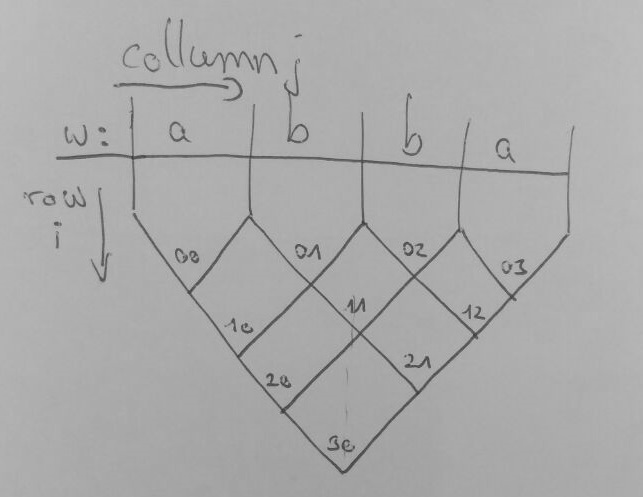
\includegraphics[width=0.7\textwidth]{abb/DataStructurePyramid}
\end{figure}

 \pagebreak 
 
\frame{
	\begin{algorithm}[H] %or another one check
		\caption{distributeRhseRandomly}
		\label{distributeRhseRandomly}
		\SetAlgoLined
		\KwIn{ $G,\ Rhse \subseteq\ RHSE,\ 0\leq minCount\leq maxCount\leq \mid G.V\mid$}
		\KwOut{$Grammar\ G\ with\ randomly\ distributed\ Rhse's.$}
		\ForEach {$rhse\ in\ Rhse$}{
			$addCount$ = $random(minCount, maxCount)$\;
			$VarsToAddTo = randomSubSet(addCount,\ LHSE)$\;
			
		
			\ForEach{var in VarsToAddTo}{
				$G.P = G.P\ \cup\ \{ "var\longrightarrow rhse" \} $\;	
			}
		}
		\Return $G$;
	\end{algorithm}
}
.\\
.\\
\frame{
	\begin{algorithm}[H] %or another one check
		\caption{GeneratorGrammarDiceRollMartens}
		\label{GeneratorGrammarDiceRollMartens}
		\SetAlgoLined
		\KwIn{ $word \in \Sigma^{*},\ V,\ \Sigma,\ S,\ P = \emptyset,\ minCount\Sigma,\ maxCount\Sigma,\ $ $ minCountVarComp,\ maxCountVarComp $ }
		\KwOut{$G$}
		
		$G=(V,\Sigma , S, P)$\;
		$G = distributeRhseRandomly(G,\ \Sigma,\ minCount\Sigma,\ maxCount\Sigma ) $\;
		$pyramid = CYK.calculatePyramid(G,\ word)$\;
		\ForEach{$cell_{i+1,j}\ in\ pyramid\ \wedge\ i>0$}{
			$VarComp = \{XY\ |\ X \in cellUpperLeft\ \wedge\ Y \in cellUpperRight \}$\;
			\ForEach{$vc\ in\ VarComp$}{
				\While{$cell_{wordLength+1,0} = \emptyset$}{
					$distributeRhseRandomly(G,\ vc,\ minCountVarComp,\ $ $maxCountVarComp ) $\;
					$pyramid = CYK.calculatePyramid(G,\ word)$\;	
				}
			}
		}
		\Return $G$\;
		\footnotetext{Line 3: Fills the i=0 row of the pyramid.\\
			\noindent Line 4: = foreach cellDown, but skipping the first row of the pyramid.
		}
	\end{algorithm}
}

 \pagebreak 
 
 
\frame{
 	\begin{algorithm}[H] %or another one check
 		\caption{checkRightCellCombination}
 		\label{checkRightCellCombination}
 		\SetAlgoLined
 		\KwIn{$ cellDown\subseteq V \,\ cellUpperLeft\subseteq V,\ cellUpperRight\subseteq V,\ G.P $ }
 		\KwOut{$varsThatForce\subseteq V$}
 		$isForced = false$\;
 		$VarsThatForce = \emptyset$\;
 		$VarComp = \{XY\ |\ X \in cellUpperLeft\ \wedge\ Y \in cellUpperRight \}$\;
 		\ForEach{$v\ in\ cellDown$}{
 			$VProd = \{p\ |\ p \in G.P\ \wedge\ p.lhse = v \}$\;
 			$VRhse = \{vRhse\ |\ vRhse \in VProd.RHSE \} $\;
 			\If{$VarComp \nsubseteq VRhse$}{
 				$isForced = true$\;
 				$VarsThatForce = VarsThatForce\ \cup\ v$\;
 			}			
 		}
 		\Return $VarsThatForce$\;
 	\end{algorithm}
}
\pagebreak


\frame{
 	\begin{algorithm}[H] %or another one check
 		\caption{checkRightCellCombinationForced}
 		\label{checkRightCellCombinationForced}
 		\SetAlgoLined
 		\KwIn{$ pyramid,\ G,\ minCountForced $ }
 		\KwOut{$G$}
 		$countForced = 0$\;
 		$isForced = true$\;
 		$varsThatForce = empty\ pyramid$\;
 		\ForEach{$cell_{i+1,j}\ in\ pyramid\ \wedge\ i>1 $}{
 			$varComp = \{XY\ |\ X\ \epsilon\ Cell_{i,j}\ \wedge\ Y\ \epsilon\ Cell_{i+1,j+1} \}$\;
 			
 			
 			
 			$ $\;
 		}
 		\Return $isForced,\ countForced,\ varsThatForce$\;
 		\footnotetext{Line 3: $i>1 \rightarrow$ the upper two rows aren't included, because they would produce trivial cases that fulfil the restriction always. 
 		}
 	\end{algorithm}
}
 
\pagebreak
 
\lstset{language=java}
\begin{lstlisting}[frame=htrbl, caption={distributeDiceRollRightHandSideElements}, 
label={lst:distributeDiceRollRightHandSideElements}]
Algorithm: distributeDiceRollRightHandSideElements
Input: grammar, setRhse, minCount, maxCount, listVars;
Output: grammar;

for(RightHandSideElement rhse : setRhse){
	// countWillBeAdded is between [minCount, maxCount]. 
	countWillBeAdded = diceRoll();
	while(listVars.size() > countWillBeAdded){
		Remove one variable of listVars via dice roll;
	}
	for(Variable varLeft : listVars){
		// An exception is thrown if the production 
		// already exists.
		grammar.addProduction "varLeft --> rhse";
	}
}
return grammar;
\end{lstlisting}


\lstset{}
\begin{lstlisting}[frame=htrbl, caption={distributeDiceRollRightHandSideElementsShort}, 
label={lst:distributeDiceRollRightHandSideElementsShort}]
Algorithm: distributeDiceRollRightHandSideElements
Input: grammar G, setRhse, minCount, maxCount, setGrammarVars;
Output: grammar;

foreach rhse in setRhse { 
	countWillBeAdded = dice roll a number within [minCount, maxCount];
	setVarsToAddRhse = {}dice roll countWillbeAdded to times vars from 	
		setGrammarVars that get the rhse added to;
	foreach var in setVarsToAddRhse {
		add production "var --> rhse" to grammar;
	}
}
return grammar;
\end{lstlisting}

\lstset{language=java}
\begin{lstlisting}[frame=htrbl, caption={CYK.calculateSetVAdvanced}, 
label={lst:CYK.calculateSetVAdvanced}]
Algorithm: CYK.calculateSetVAdvanced
Input: grammar, word;
Output: Set<VariableK>[][] cYKMatrix;

Set<VariableK>[][] cYKMatrix = new Set<VariableK>[wordSize][wordSize];
cYKMatrix = calculateCYKMatrix;
return cYKMatrix;
\end{lstlisting}

\pagebreak

\lstset{language=java}
\begin{lstlisting}[frame=htrbl,caption={GeneratorGrammarDiceRollTopDownMartens}, 
label={lst:GeneratorGrammarDiceRollTopDownMartens}]
Algorithm: GeneratorGrammarDiceRollTopDownMartens
Input: word, settings;
Output: grammar;
Note: Keep in mind that the setV matrix is a upper right matrix. But the
description of how the algorithm works is done, as if the setV pyramid 
points downwards (reflection on the diagonal + rotation to the left).
Regarding one cell, its upper left cell and its upper right cell 
are looked at. setV[i][j] = down cell. setV[i + 1][j] = upper right cell
setV[i][j - 1] = upper left cell. With wordSize = 5, the visited indexes 
are as following: [01->12->23->34; 02->13->24; 03->14; 04;]

Grammar grammar = new Grammar();
// Part1: Distribute the terminals.
grammar = distributeDiceRollRightHandSideElements(
	grammar, settingsTerminals, minCountTerminals, 
	maxCountTerminals, settingsListVariables);
// Part2: Distribute the compound variables.
Set<VariableKWrapper>[][] setVAdvanced;
// Fill the diagonal of the matrix with:
setVAdvanced = CYK.calculateSetVAdvanced( grammar, word );
for(Cell cellToBeVisited : setVAdvanced){
	setVariableCompound = calculate all the possible tupels of 
		({varLeft}, {varRight});
	for(VariableCompound varComp : setVariableCompound){
		// Because of dice rolling anyways and lots of grammars 
		// being generated, no varComp is added if the production
		// already exists.
		grammar = distributeDiceRollRightHandSideElements(
			grammar, varComp, minCountVarComp, 
			maxCountVarComp, settingsListVariables);
		setVAdvanced = CYK.calculateSetVAdvanced( grammar, word );
	}
}
return grammar;
// Forgot the while cell not empty do this from line 21 to line 33;
\end{lstlisting}

\pagebreak

\lstset{language=java}
\begin{lstlisting}[frame=htrbl,caption={GeneratorGrammarDiceRollOnly}, 
label={lst:GeneratorGrammarDiceRollOnly}]
Algorithm: GeneratorGrammarDiceRollOnly
Input: settings;
Output: grammar;
Note: A lot of productions are generated, that later on are not needed
for parsing the specific word.

Grammar grammar = new Grammar();
// Part1: Distribute the terminals.
grammar = distributeDiceRollRightHandSideElements(
	grammar, settingsTerminals, minCountTerminals, 
	maxCountTerminals, settingsListVariables);
// Part2: Distribute the compound variables.
Set<Variables> vars = settings.getVariables();
Set<VariablesCompound> setVarComp;
setVarComp = calculate all the possible tupels of ({vars}, {vars});
grammar = distributeDiceRollRightHandSideElements(
	grammar, settingsTerminals, minCountVariableCompound, 
	maxCountVariableCompound, setVarComp);
return grammar
\end{lstlisting}

\pagebreak

\lstset{language=java}
\begin{lstlisting}[frame=htrbl,caption={GeneratorGrammarDiceRollOnlyBias}, 
label={lst:GeneratorGrammarDiceRollOnlyBias}]
Algorithm: GeneratorGrammarDiceRollOnlyBias
Input: settings;
Output: grammar;
Note: A lot of productions are generated, that later on are not needed
for parsing the specific word.

Grammar grammar = new Grammar();
// Distribute the terminals.
grammar = distributeDiceRollRightHandSideElementsBias(
	grammar, settingsTerminals, settingsMinCountTerminals, 
	settingsMCountTerminals, settingsListVars, settingsFavouritism);

// Distribute the compound variables.
Set<VariablesCompound> setVarComp;
setVarComp = calculate all the possible tupels of ({vars}, {vars});
grammar = distributeDiceRollRightHandSideElementsBias(
	grammar, varComp, settingsMinCountVars,
	settingsMaxCountVars, settingsListVars, settingsFavouritism);
return grammar;
\end{lstlisting}

\pagebreak

\lstset{language=java}
\begin{lstlisting}[frame=htrbl,caption={distributeDiceRollRightHandSideElementsBias}, 
label={lst:distributeDiceRollRightHandSideElementsBias}]
Algorithm: distributeDiceRollRightHandSideElementsBias
Input: grammar, setRhse, minCount, maxCount, listVars, favouritismList;
Output: grammar;
Note: Because of dice rolling anyways and lots of grammars being 
generated, no rhse is added if the production already exists.

// Calculate the bloated varSet.
List<Variable> varsBloated;
for(Variables varTemp :  settings.getVariables()){
	tempFavour = randomly pick favouritism[i];
	varsBloated.add({tempFavour times varTemp});
	favouritism.remove(tempFavour);
}
// Because of dice rolling anyways and lot of grammars being generated, 
// just no rhse is added if the production already exists.
grammar = distributeDiceRollRightHandSideElements( grammar,
	varsBloated, minCount, maxCount, listVars );
return grammar;
\end{lstlisting}

\frame{
	\begin{algorithm}[H] %or another one check
		\caption{distributeDiceRollRightHandSideElementsBias}
		\label{distributeDiceRollRightHandSideElementsBias}
		\SetAlgoLined
		\KwIn{ $G,\ rhse \subseteq\ RHSE,\ 0\leq minCount\leq maxCount\leq\ \mid G.V\mid,\ favouritism = \{x\ |\ x\ \epsilon\ \mathrm{N}\ \wedge\ |favouritism| = |G.V| \}$}
		\KwOut{$G$}
		
		$favour = \{(v,\ f )\ |\ v\ \epsilon\ V \wedge\ f\ \epsilon\ favouritism\  \wedge\ tupel\ are\ created\ via\ dice\ roll \}$\;
		$varsBloated_b = \emptyset $\;
		\ForEach{fav in favour}{
			$varsBloated_b = varsBloated_b\ \biguplus\ \{ v^{f} \}$\;
		}
		\Return $distributeDiceRollRhse(
		G ,\ MISTAKEHEREvarsBloated_b,\ minCount,\ maxCount\ )$\;
		
		Still working on. One more Pprameter needed for distributeDiceRollRighthandSideElement. Parameter V that defines the variables the rhse are added to. OR make this algorithm independent.
		\footnotetext{Line 6: Note that $varsBloated_b$ is a multiset, but should actually be a set. Exceptions causing a duplicate production to
		the grammar are not relevant because G.P is a set. }
	\end{algorithm}
}

\pagebreak
\noindent Description of the checks here. \\
\noindent All test of the GrammarValidityChecker class are based on the simple setV matrix. \\

\noindent  isValid = isWordProducible \&\& isExamConstraints \&\& isGrammarRestrictions\\

\noindent  isWordProducible = CYK.algorithmAdvanced()\\

\noindent  isExamConstraints = isRightCellCombinationsForced \&\& isMaxSumOfProductionsCount \&\& isMaxSumOfVarsInPyramidCount \&\& countRightCellCombinationsForced \\

\noindent isGrammarRestrictions = isSizeOfWordCount \&\& isMaxNumberOfVarsPerCellCount \\

\lstset{language=java}
\begin{lstlisting}[frame=htrbl, caption={checksumOfProductions}, 
label={lst:checksumOfProductions}]
Algorithm: checksumOfProductions
Input: grammar, maxSumOfProduction;
Output: isSumOfProductions;

return grammar.getProductionsAsList().size() <= maxSumOfProductions; 
\end{lstlisting}

\pagebreak
\lstset{language=java}
\begin{lstlisting}[frame=htrbl, caption={checkMaxNumberOfVarsPerCell}, 
label={lst:checkMaxNumberOfVarsPerCell}]
Algorithm: checkMaxNumberOfVarsPerCell
Input: setVSimple, maxNumberOfVarsPerCell;
Output: isMaxNumberOfVarsPerCell;
Note: Checking for maxNumberOfVarsPerCell <= zero isn't allowed;

int tempMaxNumberOfVarsPerCell = 0;
int wordLength = tempSetV[0].length;
for ( int i = 0; i < wordLength; i++ ) {
	for ( int j = 0; j < wordLength; j++ ) {
		if ( tempSetV[i][j].size() > numberOfVarsPerCell ) {
			numberOfVarsPerCell = tempSetV[i][j].size();
		}
	}
}
return tempMaxNumberOfVarsPerCell <= maxNumberOfVarsPerCell;
\end{lstlisting}

\pagebreak

\lstset{language=java}
\begin{lstlisting}[frame=htrbl, caption={checkMaxSumOfVarsInPyramid}, 
label={lst:checkMaxSumOfVarsInPyramid}]
Algorithm: checkMaxSumOfVarsInPyramid
Input: setVSimple, maxSumOfVarsInPyramid;
Output: isMaxSumOfVarsInPyramid;

// put all vars of the matrix into one list and use its length.
List<Varaible> allVarsList = new ArrayList<>();
for ( int i = 0; i < setVSimple.length; i++ ) {
	for ( int j = 0; j < setVSimple.length; j++ ) {
		tempVars.addAll( setVSimple[i][j] );
	}
}
return allVarsList.size() <= maxSumOfVarsInPyramid; 
\end{lstlisting}

\pagebreak

\lstset{language=java}
\begin{lstlisting}[frame=htrbl, caption={rightCellCombinationsForced}, 
label={lst:rightCellCombinationsForced}]
Algorithm: rightCellCombinationsForced
Input: setVSimple, minCountForced, grammar;
Output: isForced, countForced, setVSimpleVarsThatForce;
Note: Keep in mind that the setV matrix is a upper right matrix. But the
description of how the algorithm works is done, as if the setV pyramid 
points downwards (reflection on the diagonal + rotation to the left).
Regarding one cell, its upper left cell and its upper right cell 
are looked at. setV[i][j] = down cell. setV[i + 1][j] = upper right cell
setV[i][j - 1] = upper left cell.

int countForced = 0;
Set<Variable>[][] setVMarkedVarsThatForce;
for(Cell cell : setVSimple){
	// Trivial cases that would fulfil the restrictions each time. 
	Ignore the upper two rows of the pyramid; 
	isRightCellCombinationForced = true;
	if(!upperLeftCell.isEmpty() && !upperRightCell.isEmpty()) {
		break;
	}
	setVariableCompound = calculate all the possible tupels of 
		({varLeft}, {varRight});
	for(Variable var : cellToBeVisited) {
		varDownProdList = grammar.getProdList(varDown);
		for(VariableCompound varComp : setVariableCompound) {
			for(Production prod : varDownProdList){
				if(prod.getRhse() == varComp) {
					isForced = false;
				}
			}
		}
		if(isRightCellCombinationForced) {
			rightCellCombinationsForced++;
			// Cell has index i and j.
			setVMarkedVarsThatForce[i][j].add(var)
		}
	}
}
boolean isForced = countForced >= minCountRightCellCombinationsForced;
return isForced, countForced, setVMarkedVarsThatForce;
\end{lstlisting}

\pagebreak

\lstset{language=java}
\begin{lstlisting}[frame=htrbl, caption={Util.removeUselessProductions}, 
label={lst:Util.removeUselessProductions}]
Algorithm: Util.removeUselessProductions
Input: grammar, setVSimple, word
Output: grammar
Note: Very similar to the calculateSetVAdvanced algorithm. Additionally
to storing the k, it is also saved, which production have been used. 
All productions that haven't been need are removed, from the grammar.

Set<Production> allProductions = grammar.getProductions();
Set<Production> onlyUsefulProductions;
onlyUsefulProductions = calculate useful productions with the input of
	grammar, setVSimple and word ;
grammar.remove(allProductions);
return grammar.add(onlyUsefulProductions);
\end{lstlisting}

\pagebreak

% evtl. Anhang
%\newpage
%\addcontentsline{toc}{section}{Listings}
%\fancyhead[L]{Listings} %Kopfzeile links
%\section*{Listings}

Following are some interesting classes referenced in the thesis that were too long to fit into the text.
\\

\noindent
\textbf{Transaction}:\\
This class is the simple Transaction representation used to control index changes. It is not intended to be similar to a RDBMS transaction, but is merely a batch context with simple commit and rollback features.
\\
\lstset{language=java}
\begin{lstlisting}[frame=htrbl, caption={the simple Transaction contract}, label={lst:Transaction.java}]
public class Transaction implements TransactionContext {

	private boolean progress = true;
	private List<Synchronization> syncs = new ArrayList<>();
	
	@Override
	public boolean isTransactionInProgress() {
		return this.progress;
	}
	
	@Override
	public Object getTransactionIdentifier() {
		return this;
	}
	
	@Override
	public void registerSynchronization(
		Synchronization synchronization ) {
		this.syncs.add( synchronization );
	}
	
	/**
	 * @throws IllegalStateException if already commited/rolledback
	 */
	public void commit() {
		if ( !this.progress ) {
			throw new IllegalStateException( 
			"can't commit - " + 
			"No Search Transaction is in Progress!" );
		}
		this.progress = false;
		this.syncs.forEach( Synchronization::beforeCompletion );
		
		for ( Synchronization sync : this.syncs ) {
			sync.afterCompletion( Status.STATUS_COMMITTED );
		}
	}
	
	/**
	 * @throws IllegalStateException if already commited/rolledback
 	 */
	public void rollback() {
		if ( !this.progress ) {
			throw new IllegalStateException( 
			"can't rollback - " + 
			"No Search Transaction is in Progress!" );
		}
		this.progress = false;
		this.syncs.forEach( Synchronization::beforeCompletion );
	
		for ( Synchronization sync : this.syncs ) {
			sync.afterCompletion( Status.STATUS_ROLLEDBACK );
		}
	}

}
\end{lstlisting}

\pagebreak

\noindent
\textbf{StandaloneSearchConfiguration}:\\
hibernate-search-engine requires an object implementing the SearchConfiguration interface. StandaloneSearchConfiguration is the basic implementation of this used in our standalone version of Hibernate Search.
\\
\lstset{language=java}
\begin{lstlisting}[frame=htrbl, caption={StandaloneSearchConfiguration.java}, label={lst:StandaloneSearchConfiguration.java}]
/**
 * Manually defines the configuration. 
 * Classes and properties are the only implemented options at the moment.
 *
 * @author Martin Braun (adaption), Emmanuel Bernard
 */
public class StandaloneSearchConfiguration 
	extends SearchConfigurationBase 
	implements SearchConfiguration {

	private final Logger LOGGER = 
		Logger.getLogger( 
			StandaloneSearchConfiguration.class.getName() 
		);
		
	private final Map<String, Class<?>> classes;
	private final Properties properties;
	private final HashMap<Class<? extends Service>, Object> 
		providedServices;
	private final InstanceInitializer initializer;
	private SearchMapping programmaticMapping;
	private boolean transactionsExpected = true;
	private boolean indexMetadataComplete = true;
	private boolean idProvidedImplicit = false;
	private ClassLoaderService classLoaderService;
	private ReflectionManager reflectionManager;

	public StandaloneSearchConfiguration() {
		this( new Properties() );
	}

	public StandaloneSearchConfiguration(Properties properties) {
		this( 
			SubClassSupportInstanceInitializer.INSTANCE, 
			properties
		);
	}

	public StandaloneSearchConfiguration(InstanceInitializer init) {
		this( new Properties() );
	}

	public StandaloneSearchConfiguration(InstanceInitializer init, 
		Properties properties) {
		this.initializer = init;
		this.classes = new HashMap<>();
		this.properties = properties;
		// default values if nothing was explicitly set
		this.properties.computeIfAbsent(
			"hibernate.search.default.directory_provider", 
			(key) -> {
				LOGGER.info( 
				  "defaulting to RAM directory-provider" 
				);
			return "ram";
		});
		this.properties.computeIfAbsent(
			"hibernate.search.lucene_version", 
			(key) -> {
				LOGGER.info( 
					"defaulting to Lucene Version: " 
					+ Version.LUCENE_5_2_1.toString() 
				);
				return Version.LUCENE_5_2_1.toString();
		});
		this.reflectionManager = new JavaReflectionManager();
		this.providedServices = new HashMap<>();
		this.classLoaderService = new DefaultClassLoaderService();
	}

	public StandaloneSearchConfiguration addProperty(String key,
		String value) {
		properties.setProperty( key, value );
		return this;
	}

	public StandaloneSearchConfiguration addClass(Class<?> indexed) {
		classes.put( indexed.getName(), indexed );
		return this;
	}

	@Override
	public Iterator<Class<?>> getClassMappings() {
		return classes.values().iterator();
	}

	@Override
	public Class<?> getClassMapping(String name) {
		return classes.get( name );
	}

	@Override
	public String getProperty(String propertyName) {
		return properties.getProperty( propertyName );
	}

	@Override
	public Properties getProperties() {
		return properties;
	}

	@Override
	public ReflectionManager getReflectionManager() {
		return this.reflectionManager;
	}

	@Override
	public SearchMapping getProgrammaticMapping() {
		return programmaticMapping;
	}

	public StandaloneSearchConfiguration setProgrammaticMapping(
			SearchMapping programmaticMapping
		) {
		this.programmaticMapping = programmaticMapping;
		return this;
	}

	@Override
	public Map<Class<? extends Service>, Object> 
		getProvidedServices() {
		return providedServices;
	}

	public void addProvidedService(
			Class<? extends Service> serviceRole,
			Object service
		) {
		providedServices.put( serviceRole, service );
	}

	@Override
	public boolean isTransactionManagerExpected() {
		return this.transactionsExpected;
	}

	public void setTransactionsExpected(
			boolean transactionsExpected) {
		this.transactionsExpected = transactionsExpected;
	}

	@Override
	public InstanceInitializer getInstanceInitializer() {
		return initializer;
	}

	@Override
	public boolean isIndexMetadataComplete() {
		return indexMetadataComplete;
	}

	public void setIndexMetadataComplete(
		boolean indexMetadataComplete) {
		this.indexMetadataComplete = indexMetadataComplete;
	}

	@Override
	public boolean isIdProvidedImplicit() {
		return idProvidedImplicit;
	}

	public StandaloneSearchConfiguration 
		setIdProvidedImplicit(boolean idProvidedImplicit) {
		this.idProvidedImplicit = idProvidedImplicit;
		return this;
	}

	@Override
	public ClassLoaderService getClassLoaderService() {
		return classLoaderService;
	}

	public void setClassLoaderService(
		ClassLoaderService ) {
		this.classLoaderService = classLoaderService;
	}

}
\end{lstlisting}

\pagebreak

\noindent
\textbf{BasicEntityProvider}:\\
This is the basic implementation of the EntityProvider interface which is used to abstract the database access in the standalone version. It uses a JPA EntityManager to accomplish this.
\\
\lstset{language=java}
\begin{lstlisting}[frame=htrbl, caption={BasicEntityProvider.java}, label={lst:BasicEntityProvider.java}]
public class BasicEntityProvider implements EntityProvider {

	private static final String QUERY_FORMAT = 
		"SELECT obj FROM %s obj " +
		"WHERE obj.%s IN :ids";
	private final EntityManager em;
	private final Map<Class<?>, String> idProperties;

	public BasicEntityProvider(EntityManager em,
		Map<Class<?>, String> idProperties) {
		this.em = em;
		this.idProperties = idProperties;
	}

	@Override
	public void close() throws IOException {
		this.em.close();
	}

	@Override
	public Object get(Class<?> entityClass, Object id,
		Map<String, String> hints) {
		return this.em.find( entityClass, id );
	}

	@SuppressWarnings({"rawtypes", "unchecked"})
	@Override
	public List getBatch(Class<?> entityClass, List<Object> ids,
		Map<String, String> hints) {
		List<Object> ret = new ArrayList<>( ids.size() );
		if ( ids.size() > 0 ) {
			String idProperty = 
				this.idProperties.get( entityClass );
			String queryString = 
				String.format(
					QUERY_FORMAT,
					this.em.getMetamodel()
						.entity( entityClass )
						.getName(),
					idProperty
		);
		Query query = this.em.createQuery( queryString );
		query.setParameter( "ids", ids );
			ret.addAll( query.getResultList() );
		}
		return ret;
	}
	
	public void clearEm() {
		this.em.clear();
	}

	public EntityManager getEm() {
		return this.em;
	}

}
\end{lstlisting}

\pagebreak

\noindent
\textbf{Obtaining the idProperties}:\\
This code snippet shows how the idProperties map needed for the instantiation of a BasicEntityProvider can be obtained. This mechanism is used on some other places of Hibernate Search GenericJPA as well.
\\
\lstset{language=java}
\begin{lstlisting}[frame=htrbl, caption={Obtaining idProperties}, label={lst:idProperties.java}]
SearchConfiguration config = ...;

MetadataProvider metadataProvider = 
	MetadataUtil.getDummyMetadataProvider( config );
MetadataRehasher rehasher = new MetadataRehasher();

List<RehashedTypeMetadata> rehashedTypeMetadatas = new ArrayList<>();
for ( Class<?> indexRootType : this.getIndexRootTypes() ) {
	RehashedTypeMetadata rehashed = 
		rehasher.rehash( 
			metadataProvider
				.getTypeMetadataFor( indexRootType ) 
		);
	rehashedTypeMetadatas.add( rehashed );
}

Map<Class<?>, String> idProperties = 
	MetadataUtil.calculateIdProperties( rehashedTypeMetadatas );
\end{lstlisting}

\pagebreak

\noindent
\textbf{MultiQueryAccess}:\\
This is the utility class used to scroll results from multiple queries at once while retrieving the events from the database in the asynchronous approach.
\\
\lstset{language=java}
\begin{lstlisting}[frame=htrbl, caption={MultiQueryAccess.java}, label={lst:MultiQueryAccess.java}]
/**
 * Utility class that allows you to access multiple JPA queries at once.
 * Data is retrieved from the database in batches
 * and ordered by a given comparator.
 * No need for messy Unions on the database level! <br>
 * <br>
 * This is particularly useful if you scroll all the data 
 * from the database incrementally and if you can 
 * compare in Code.
 *
 * @author Martin
 */
public class MultiQueryAccess {

	private final Map<String, Long> currentCountMap;
	private final Map<String, Query> queryMap;
	private final Comparator<ObjectIdentifierWrapper> comparator;
	private final int batchSize;
	
	private final Map<String, Long> currentPosition;
	private final Map<String, LinkedList<Object>> values;
	
	private Object scheduled;
	private String identifier;


	public MultiQueryAccess(
		Map<String, Long> countMap,
		Map<String, Query> queryMap,
		Comparator<ObjectIdentifierWrapper> comparator,
		int batchSize) {
		if ( countMap.size() != queryMap.size() ) {
			throw new IllegalArgumentException( 
				"countMap.size() must be equal " + 
					"to queryMap.size()" );
		}
		this.currentCountMap = countMap;
		this.queryMap = queryMap;
		this.comparator = comparator;
		this.batchSize = batchSize;
		this.currentPosition = new HashMap<>();
		this.values = new HashMap<>();
		for ( String ident : queryMap.keySet() ) {
			this.values.put( ident, new LinkedList<>() );
			this.currentPosition.put( ident, 0L );
		}
	}

	private static int toInt(Long l) {
		return (int) (long) l;
	}

	/**
	 * increments the value to be returned by {@link #get()}
	 *
	 * @return true if there is a value left to be visited 
	 *	in the database
	 */
	public boolean next() {
	
	/*
	 *
	 *
	 * indentation broken to make this readable
	 *
	 *
	 */
	
this.scheduled = null;
this.identifier = null;
List<ObjectIdentifierWrapper> tmp =
	new ArrayList<>( this.queryMap.size() );

for ( Map.Entry<String, Query> entry : this.queryMap.entrySet() ) {
	String identifier = entry.getKey();
	Query query = entry.getValue();
	if ( !this.currentCountMap.get( identifier ).equals( 0L ) ) {
		if ( this.values.get( identifier ).size() == 0 ) {
			// the last batch is empty. get a new one
			Long processed = 
				this.currentPosition.get( identifier );
			// yay JPA...
			query.setFirstResult( toInt( processed ) );
			query.setMaxResults( this.batchSize );
			@SuppressWarnings("unchecked")
			List<Object> list = query.getResultList();
			this.values.get( identifier ).addAll( list );
		}
		Object val = this.values.get( identifier ).getFirst();
		tmp.add( new ObjectIdentifierWrapper( val, identifier ) );
	}
}
tmp.sort( this.comparator );
if ( tmp.size() > 0 ) {
	ObjectIdentifierWrapper arr = tmp.get( 0 );
	this.scheduled = arr.object;
	this.identifier = arr.identifier;
	this.values.get( this.identifier ).pop();
	Long currentPosition = this.currentPosition.get( arr.identifier );
	Long newCurrentPosition = 
		this.currentPosition
			.computeIfPresent( arr.identifier, 
				(clazz, old) -> old + 1 );
	if ( Math.abs( newCurrentPosition - currentPosition ) != 1L ) {
		throw new AssertionFailure( 
			"the new currentPosition count " + 
			"should be exactly 1 " +
			"greater than the old one" );
	}
	Long count = this.currentCountMap.get( arr.identifier );
	Long newCount = this.currentCountMap.computeIfPresent(
		arr.identifier, (clazz, old) -> old - 1
	);
	if ( Math.abs( count - newCount ) != 1L ) {
		throw new AssertionFailure( 
			"the new old remaining count " + 
				should be exactly 1 " +
				"greater than the new one" );
	}
}
return this.scheduled != null;
}

	/**
	* @return the current value
	*/
	public Object get() {
		if ( this.scheduled == null ) {
			throw new IllegalStateException(
				"either empty or next() has " + 
					"not been called" );
		}
		return this.scheduled;
	}

	/**
	* @return the identifier of the current value
	*/
	public String identifier() {
		if ( this.identifier == null ) {
			throw new IllegalStateException( 
				"either empty or next() has " + 
					"not been called" );
		}
		return this.identifier;
	}

	public static class ObjectIdentifierWrapper {
	
		public final Object object;
		public final String identifier;
		
		public ObjectIdentifierWrapper(Object object,
			String identifier) {
			this.object = object;
			this.identifier = identifier;
		}
	
	}

}
\end{lstlisting}

\pagebreak

~

%\newpage
%\addcontentsline{toc}{section}{Tables}
%\fancyhead[L]{Tables}
%\section*{Tables}
This section contains all tables referenced in this thesis.
\\

\noindent
\textbf{JPASearchFactoryController configuration}:\\
When instantiating the JPASearchFactoryController with the Setup class the developer has to pass a property-Map (or a Java Properties) object. Besides containing the hibernate-search-engine configuration properties, some Hibernate Search GenericJPA configuration properties can be set in this map as well:
\\
\begin{table}[h] 
	\centering
	\begin{tabular}{|c|c|}
		\hline 
		hibernate.search.useJTATransactions & \specialcell{ \textbf{false} \\ true } \\ 
		\hline 
		hibernate.search.searchfactory.type & \specialcell{ \textbf{sql} \\ manual-updates  \\ eclipselink \\ hibernate \\ openjpa} \\ 
		\hline
		hibernate.search.trigger.batchSizeForUpdates & \specialcell{ \textbf{5} } \\
		\hline
		hibernate.search.trigger.batchSizeForUpdateQueries & \specialcell{ \textbf{20} } \\
		\hline
		hibernate.search.trigger.updateDelay & \specialcell{ \textbf{200} } \\
		\hline
		hibernate.search.trigger.source & \specialcell{ <class> } \\
		\hline
		hibernate.search.additionalIndexedTypes & \specialcell{ <class>,<class>,... } \\
		\hline
		hibernate.search.transactionManagerProvider & \specialcell{
			\textbf{org.hibernate.}\\\textbf{search.generic}\\\textbf{jpa.trans}\\\textbf{action.impl}\\
			\textbf{JNDILookup}\\\textbf{Transaction}\\\textbf{ManagerProvider} 
		} \\
		\hline
		hibernate.search.transactionManagerProvider.jndi & \specialcell{ <jndi-string> } \\
		\hline
		hibernate.search.trigger.createstrategy & \specialcell{
			\textbf{create} \\
			create-drop \\
			dont-create
		} \\
		\hline
	\end{tabular}
	\footnotesize \caption{Basic JPASearchFactoryController configuration properties (\textbf{default})}
	\label{table:config_properties_jpasearchfactorycontroller}
\end{table}

\pagebreak
~

\newpage
\addcontentsline{toc}{section}{References}
\fancyhead[L]{References}
%
% ---- Bibliography ----
%
\begin{thebibliography}{100}
	
	\bibitem{jsr_jpa1} JSR 220: Enterprise Java Beans 3.0
	\url{https://jcp.org/en/jsr/detail?id=220}, 09/09/2015
	%
	
	\bibitem{javaworld_jpa1} Javaworld: Understanding JPA, Part 1
	\url{http://www.javaworld.com/article/2077817/java-se/understanding-jpa-part-1-the-object-oriented-paradigm-of-data-persistence.html}, 09/09/2015
	
	\bibitem{hibernate_orm} Hibernate ORM project homepage
	\url{http://hibernate.org/orm/}, 09/09/2015
	
	\bibitem{hibernate_search_homepage} Hibernate Search project homepage
	\url{http://hibernate.org/search/}, 09/09/2015
	
	\bibitem{hsearch_source_code_git} Hibernate Search GitHub repository
	\url{https://github.com/hibernate/hibernate-search}, 09/09/2015
	
	\bibitem{hibernate_search_faq} Hibernate Search FAQ
	\url{http://hibernate.org/search/faq/}, 09/09/2015
	
	\bibitem{lucene_apache_org} Lucene Website
	\url{https://lucene.apache.org/core/}, 09/09/2015
	
	\bibitem{elasticsearch_java_api} ElasticSearch Java API
	\url{https://www.elastic.co/guide/en/elasticsearch/client/java-api/current/index.html}, 09/09/2015
	
	\bibitem{solr_java_api} Solr Java API
	\url{https://wiki.apache.org/solr/Solrj}, 09/09/2015
	
	\bibitem{xkcd_competing_standards_source} xkcd \#927 on competing standards
	\url{https://xkcd.com/927/}, 09/09/2015
	
	\bibitem{top_down_strandh} Top-down programming, Robert Strandh
	\url{http://dept-info.labri.fr/~strandh/Teaching/PFS/Common/Strandh-Tutorial/top-down-programming.html},
	09/09/2015
	
	\bibitem{bottom_up_strandh} Bottom-up programming, Robert Strandh
	\url{http://dept-info.labri.fr/~strandh/Teaching/PFS/Common/Strandh-Tutorial/bottom-up-programming.html},
	09/09/2015
	
	\bibitem{singleresponsibility_objectmentor} objectmentor.com: Article on Single Responsibility Principle
	\url{http://www.objectmentor.com/resources/articles/srp.pdf}, 09/09/2015
	
	\bibitem{openclosed_objectmentor} objectmentor.com: Article on Open-Closed-Principle
	\url{http://www.objectmentor.com/resources/articles/ocp.pdf}, 09/09/2015
	
	\bibitem{openclosed_bertrand} Object-Oriented Software Construction, Prentice Hall, 1988, Bertrand Meyer
	
	\bibitem{maven_homepage} Maven project homepage
	\url{https://maven.apache.org/}, 09/09/2015
	
	\bibitem{jdbc_oracle} Oracle JDBC overview
	\url{http://www.oracle.com/technetwork/java/javase/jdbc/index.html}, 09/09/2015
	
	\bibitem{oledb_ms} Documentation on how to use OleDb with .NET
	\url{https://msdn.microsoft.com/en-us/library/5ybdbtte(v=vs.71).aspx}, 09/09/2015
	
	\bibitem{wikibooks_on_jpa} Wikibooks on Java Persistence
	\url{https://en.wikibooks.org/wiki/Java_Persistence/What_is_JPA\%3F}, 09/09/2015
	
	\bibitem{stackoverflow_jpa} Stackoverflow JPA tag
	\url{http://stackoverflow.com/tags/jpa/info}, 09/09/2015
	
	\bibitem{hibernate_ogm} Hibernate OGM project homepage
	\url{http://hibernate.org/ogm/}, 09/09/2015
	
	\bibitem{eclipselink} EclipseLink project homepage
	\url{http://www.eclipse.org/eclipselink/}, 09/09/2015
	
	\bibitem{jpa_21_jcp} JSR 338: JPA 2.1 specification
	\url{https://jcp.org/en/jsr/detail?id=338}, 09/09/2015
	
	\bibitem{openjpa} OpenJPA project homepage
	\url{http://openjpa.apache.org/}, 09/09/2015
	
	\bibitem{java_ee_spec} Java EE specification on oracle.com
	\url{http://www.oracle.com/technetwork/java/javaee/tech/index.html}, 09/09/2015
	
	\bibitem{sql_like_w3schools} w3schools on SQL LIKE
	\url{http://www.w3schools.com/sql/sql_like.asp}, 09/09/2015
	
	\bibitem{lucene_basic_concepts} Lucene Tutorial
	\url{http://www.lucenetutorial.com/basic-concepts.html}, 09/09/2015
	
	\bibitem{elasticsearch_homepage} ElasticSearch Homepage
	\url{https://www.elastic.co/products/elasticsearch}, 09/09/2015
	
	\bibitem{solr_homepage} Solr Homepage
	\url{http://lucene.apache.org/solr/}, 09/09/2015
	
	\bibitem{elasticsearch_downloads_website} ElasticSearch Download website
	\url{https://www.elastic.co/downloads/elasticsearch}, 09/09/2015
	
	\bibitem{solr_security} Solr security
	\url{https://wiki.apache.org/solr/SolrSecurity}, 09/09/2015
	
	\bibitem{elasticsearch_security} elastic Shield (security for ElasticSearch)
	\url{https://www.elastic.co/products/shield}, 09/09/2015
	
	\bibitem{solr_admin} Solr Administration (Core Specific Tools)
	\url{https://cwiki.apache.org/confluence/display/solr/Core-Specific+Tools}, 09/09/2015
	
	\bibitem{elasticsearch_admin} ElasticHQ
	\url{http://www.elastichq.org/}, 09/09/2015
	
	\bibitem{elasticsearch_clustering} ElasticSearch: Life inside a cluster
	\url{https://www.elastic.co/guide/en/elasticsearch/guide/current/distributed-cluster.html}, 09/09/2015
	
	\bibitem{solr_clustering} Solr: Introduction to Scaling and Distribution
	\url{https://cwiki.apache.org/confluence/display/solr/Introduction+to+Scaling+and+Distribution}, 09/09/2015
	
	\bibitem{hibernate_search_engine_mvnrepository} hibernate-search-engine on mvnrepository.org
	\url{http://mvnrepository.com/artifact/org.hibernate/hibernate-search-engine/5.4.0.Final}, 09/09/2015
	
	\bibitem{hibernate_search_roadmap} Hibernate Search roadmap
	\url{http://hibernate.org/search/roadmap/}, 09/09/2015
	
	\bibitem{hibernate_search_javadoc} Hibernate Search JavaDoc
	\url{https://docs.jboss.org/hibernate/search/5.5/api/}, 09/09/2015
	
	\bibitem{hibernate_search_doc} Hibernate Search documentation
	\url{http://hibernate.org/search/documentation/}, 09/09/2015
	
	\bibitem{hibernate_search_doc_massindexer} Hibernate Search documentation (MassIndexer, v5.4)
	\url{https://docs.jboss.org/hibernate/search/5.4/reference/en-US/html_single/#search-batchindex-massindexer}, 09/09/2015
	
	\bibitem{mysql_developers_lib} MySQL - Developer's Library, Fourth Edition, 2009, Paul DuBois
	
	\bibitem{postgres_triggers} CREATE TRIGGER in PostgreSQL
	\url{http://www.postgresql.org/docs/9.1/static/sql-createtrigger.html}, 09/09/2015
	
	\bibitem{hsqldb_triggers} Triggers in HSQLDB
	\url{http://hsqldb.org/doc/guide/triggers-chapt.html}, 09/09/2015
	
	\bibitem{firebird_triggers} Triggers in Firebird
	\url{http://www.firebirdsql.org/refdocs/langrefupd21-ddl-trigger.html}, 09/09/2015
	
	\bibitem{postgres_truncate} Truncate statement PostgreSQL docs
	\url{http://www.postgresql.org/docs/9.1/static/sql-truncate.html}, 09/09/2015
	
	\bibitem{firebird_conformance} Firebird conformance
	\url{http://www.firebirdsql.org/en/sql-conformance/}, 09/09/2015
	
	\bibitem{hibernate_genericjpa_github} Hibernate Search GenericJPA GitHub repository
	\url{https://github.com/Hotware/Hibernate-Search-GenericJPA}, 09/09/2015
	
	
\end{thebibliography}

%\newpage
% Erklärung
%\addcontentsline{toc}{section}{Erklärung}
%\fancyhead[L]{Erklärung}
%\section*{Erklärung}

\begin{verbatim}

\end{verbatim}

\noindent
\begin{LARGE}Erklärung zur Bachelorarbeit\end{LARGE}
\begin{verbatim}


\end{verbatim}
Ich versichere, die von mir vorgelegte Arbeit selbstständig verfasst zu haben. Alle Stellen, die wörtlich oder sinngemäß aus veröffentlichten oder nicht veröffentlichten Arbeiten anderer entnommen sind, habe ich als entnommen kenntlich gemacht. Sämtliche Quellen und Hilfsmittel, die ich für die Arbeit benutzt habe, sind angegeben. Die Arbeit hat mit gleichem Inhalt bzw. in wesentlichen Teilen noch keiner anderen Prüfungsbehörde vorgelegen.



\begin{displaymath}
% use packages: array
\begin{array}{ll}
Unterschrift:~~~~~~~~~~~~~~~~~~~~~~~~~~~~~~~~~~~~~~~~~~
& Ort, Datum:~~~~~~~~~~~~~~~~~~~~~~~~~~~~~~~~~~~~~~~~~~
\end{array}
\end{displaymath}


% leere Abschlussseite
\newpage
\thispagestyle{empty} % erzeugt Seite ohne Kopf- / Fusszeile
\section*{ }

\end{document}